\documentclass{article}

\usepackage{enumerate}
\usepackage{amssymb}
\usepackage{amsmath}
\usepackage{algorithm}
\usepackage{physics}
\usepackage{listings}
\usepackage[noend]{algpseudocode}
\usepackage{graphicx}

\graphicspath{ {./} }

\topmargin=-0.45in
\evensidemargin=0in
\oddsidemargin=0in
\textwidth=6.5in
\textheight=9.0in
\headsep=0.25in

\title{Chem 195: Problem Set 5}
\author{Michael Stephen Chen}


\begin{document}
\maketitle
\pagebreak

\section*{Problem 1}
\begin{enumerate}[i)]
  \item Please see \textbf{scf.m} for my comments
  \item Below is a plot of our estimated ground state energies using the mean field and perturbation theories. From the previous assignment, we found that the perturbation theory estimate was very accurate for low anharmonic factors (at least up until $a=0.1$). This is because for weak perturbations, the change in energy is roughly linear. The similarity between our mean field and perturbation estimates likewise show that the mean field approach is fairly accurate. Also mean field theory appears to, at least qualitatively, account for the nonlinearity of the perturbation (unlike our linear perturbation estimates) as the plot appears to level off with larger $a$ values.

    \begin{center}
      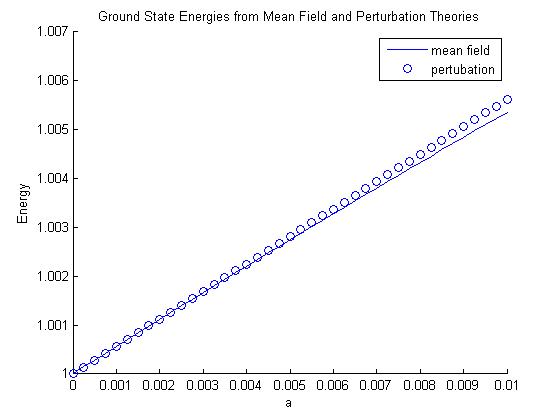
\includegraphics[scale=0.5]{prob1part2}
    \end{center}

  \item Below is a plot of ground state energies for various anharmonic factors using mean field theory.

    \begin{center}
      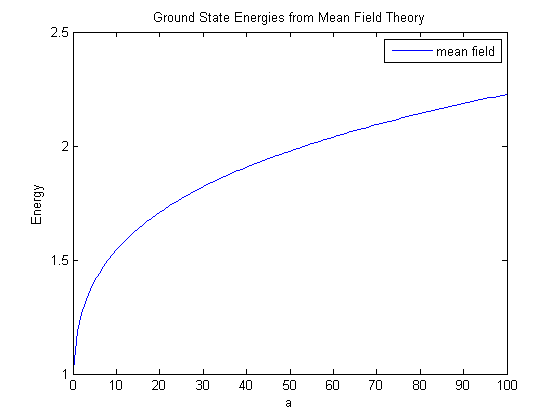
\includegraphics[scale=0.5]{prob1part3}
    \end{center}

  \item Here we plot MFT results with ``exact" values that we calculated on the previous assignment. As the anharmonic factor increases, the MFT results diverge from the exact values (which have lower energies than the corresponding values from MFT).

    \begin{center}
      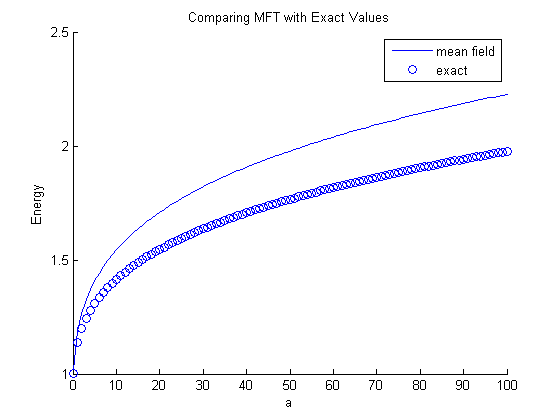
\includegraphics[scale=0.5]{prob1part4}
    \end{center}

  \item In the previous assignment, we found that the contour map for the ``exact" ground state wavefunction had a diamond-like shape (with the points of the diamond aligned aling the x- and y-axes). However our ground state, MFT contour plot has more of a boxy circle shape. The difference arises because in the exact case, our wavefunction is the result of two variable dimensions (x and y) whereas in our MFT our final wavefunction is a product of two identical 1D wavfunctions. This is because in our MFT approach, concerning the anharmonic part of the oscillator's Hamiltonian, we essentially average out the effects of one dimension. The result is a wavefunction that is more uniform.

    \begin{center}
      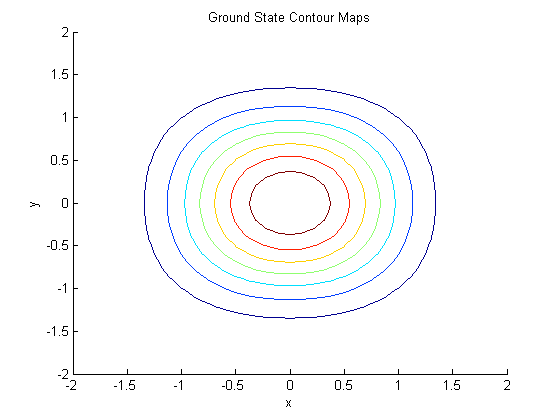
\includegraphics[scale=0.5]{prob1part5}
    \end{center}
\end{enumerate}

\section*{Problem 2}
\begin{enumerate}[i)]
  \item Please see \textbf{prob2.m}
  \item The table below displays various ground state energies for the anharmonic 2D oscillator using our "exact" method. I used a spacing of $0.5$ units between my basis functions' centers, an $\alpha=2$ for the widths, and $K=225$, which amounts to 105 basis functions after taking into account symmetry constraints.
    \begin{center}
      $\begin{array}{c|c}
        a & Energy \\ \hline
        0.000000 & 2.000000 \\ 
        0.001000 & 2.002717 \\ 
        0.010000 & 2.022490 \\ 
        0.100000 & 2.124351 \\ 
        1.000000 & 2.438472 \\ 
        10.000000 & 3.138819 \\ 
      \end{array}$
    \end{center}
  \item A scan of my work is provided below
    \begin{center}
      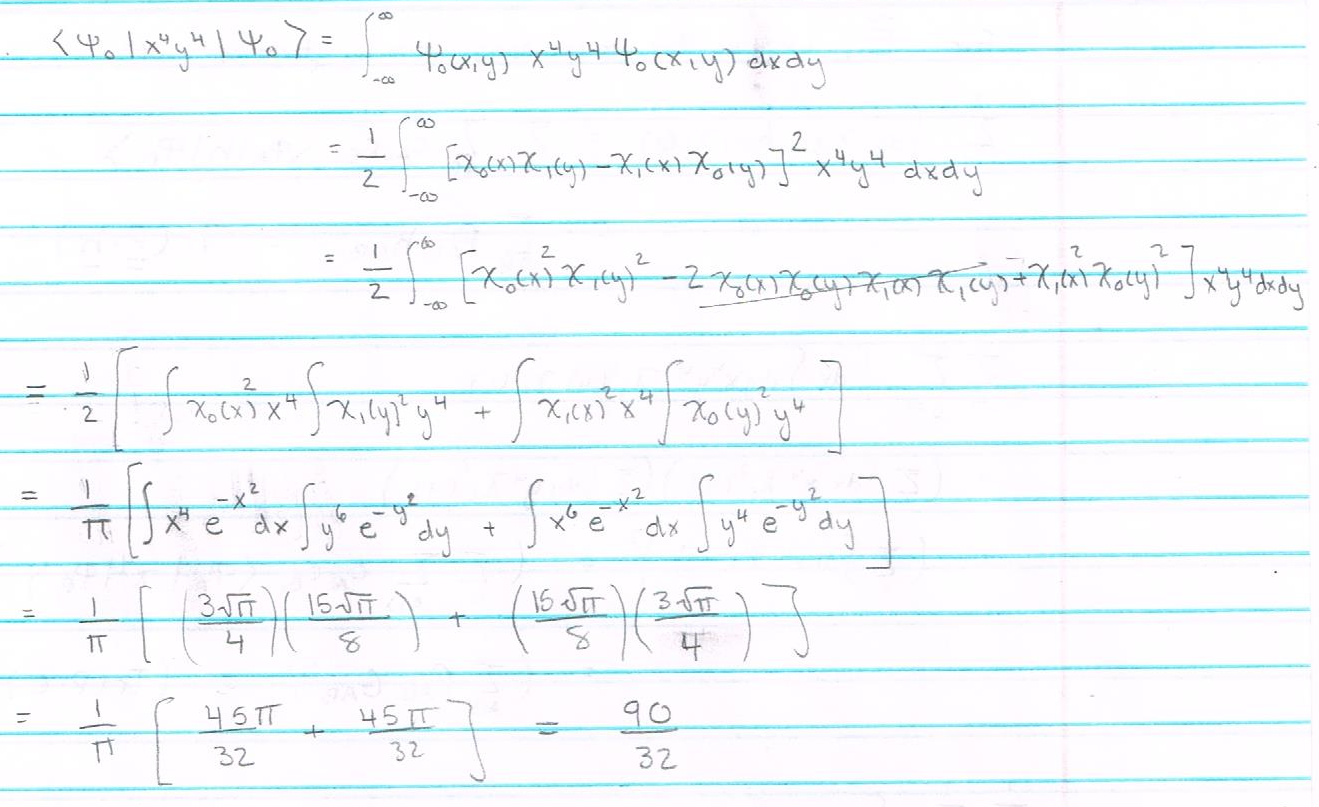
\includegraphics[scale=0.5]{prob2part3}
    \end{center}
  \item Below is a comparison of ground state energies for the perturbation and exact methods

    \begin{center}
      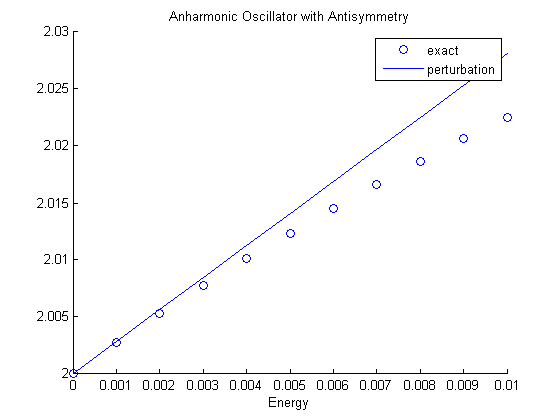
\includegraphics[scale=0.5]{prob2part4}
    \end{center}

  \item Below is the contour map for the exact ground state wavefunction
    \begin{center}
      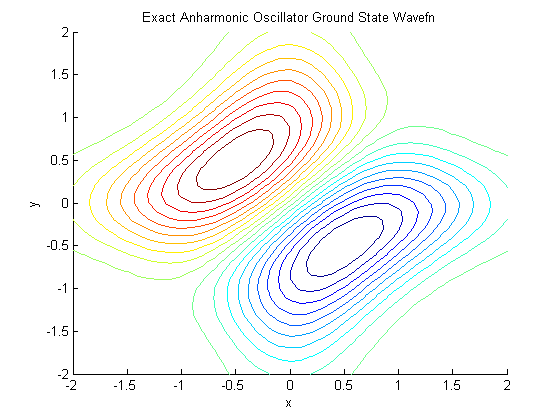
\includegraphics[scale=0.5]{prob2part5}
    \end{center}
\end{enumerate}


\section*{Problem 3}
\begin{enumerate}[i)]
  \item A scan of my work is provided below
    \begin{center}
      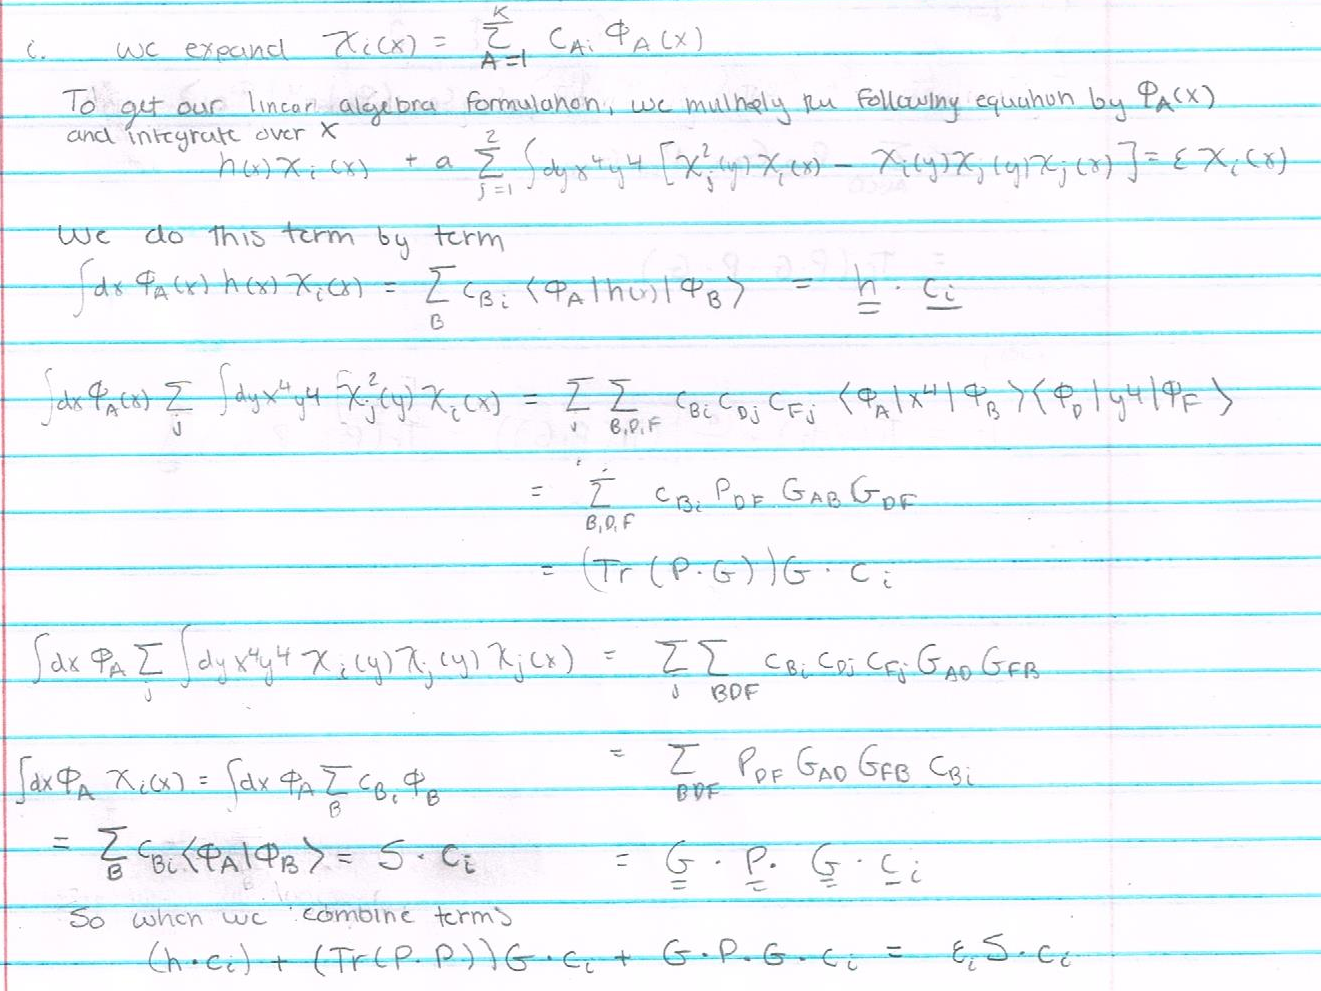
\includegraphics[scale=0.5]{prob3part1-1}

      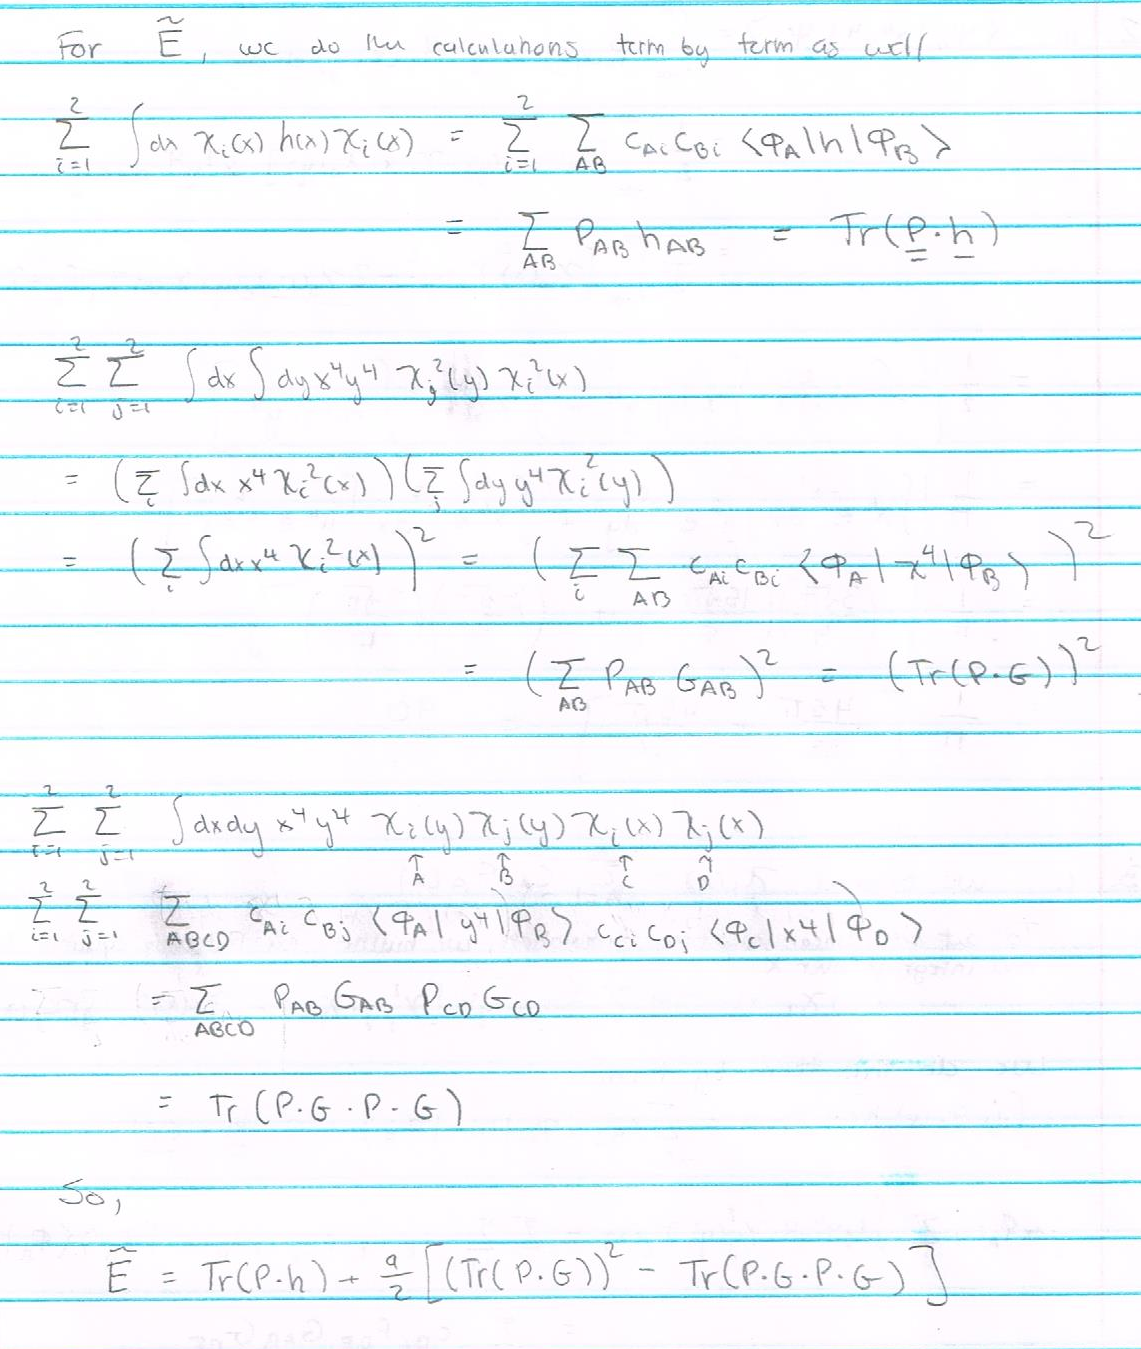
\includegraphics[scale=0.5]{prob3part1-2}
    \end{center}
  \item Below is a plot of the ground state energies of our symmetry-constrained oscillator using mean field theory
    \begin{center}
      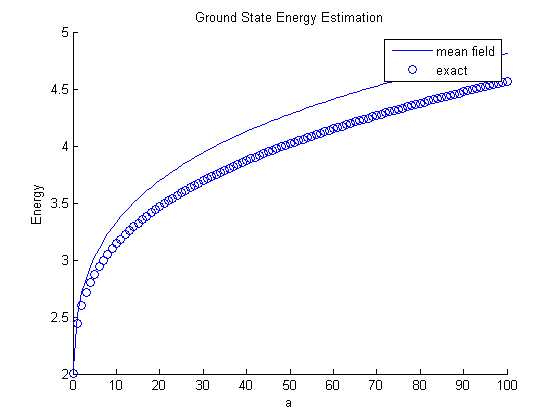
\includegraphics[scale=0.5]{prob3part2}
    \end{center}
  \item Below is the contour map for the mean field ground state wavefunction. Qualitatively, our MFT wavefunction is very similar to our exact result (namely with regard to the antisymmetry). However there are also notable differences. For instance, the exact result appears to have edges that point along the x- and y-axes, where as the MFT result does not. This is analogous to what we observe in the case where symmetry constraints are not considered (see Problem 1 part (v)).
    \begin{center}
      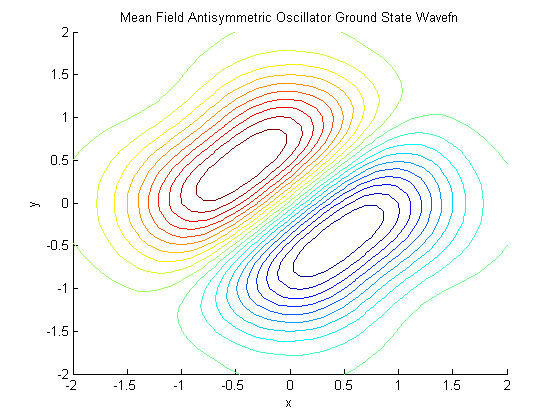
\includegraphics[scale=0.5]{prob3part3}
    \end{center}

\end{enumerate}

\end{document}
